% FlowSim slides. Build: latexmk -pdf slides.tex   Speaker notes: latexmk -pdf speaker_notes.tex
\documentclass[aspectratio=169,11pt]{beamer}
\usepackage[T1]{fontenc}
\usepackage{amsmath,amssymb,booktabs,colortbl,tikz,pgfplots,pgfplotstable}
\usetikzlibrary{arrows.meta,positioning,calc}
% Shared colours, plot styles and TikZ diagrams for slides.tex and report.tex.
\definecolor{ovgreen}{HTML}{138A07}
\definecolor{ovdark}{HTML}{0B5A04}
\definecolor{ovlight}{HTML}{E8F4E6}
\definecolor{ink}{HTML}{222222}
\definecolor{mute}{HTML}{6B6B6B}
\definecolor{today}{HTML}{E07B2A}
\definecolor{wait}{HTML}{7FBF6E}
\definecolor{late}{HTML}{C0392B}
\pgfplotsset{compat=1.18,
  fs axis/.style={axis lines=left, tick style={mute}, every axis label/.style={font=\footnotesize, color=mute},
    tick label style={font=\scriptsize, color=ink}, legend style={draw=none, font=\scriptsize, fill=none},
    axis line style={mute}, ymajorgrids, grid style={black!8}},
}
\tikzset{
  box/.style={draw=ovgreen, line width=.8pt, rounded corners=3pt, align=center, inner sep=6pt, fill=white},
  gbox/.style={box, fill=ovlight},
  arr/.style={-{Stealth[length=5pt]}, line width=.9pt, color=ovdark},
  pax/.style={circle, fill=today, minimum size=7pt, inner sep=0pt},
  lane/.style={draw=ovgreen, fill=ovlight, line width=.8pt, minimum width=1.25cm, minimum height=.55cm, rounded corners=2pt, font=\scriptsize},
}

% Single queue feeding c identical counters.
\newcommand{\queuediagram}{%
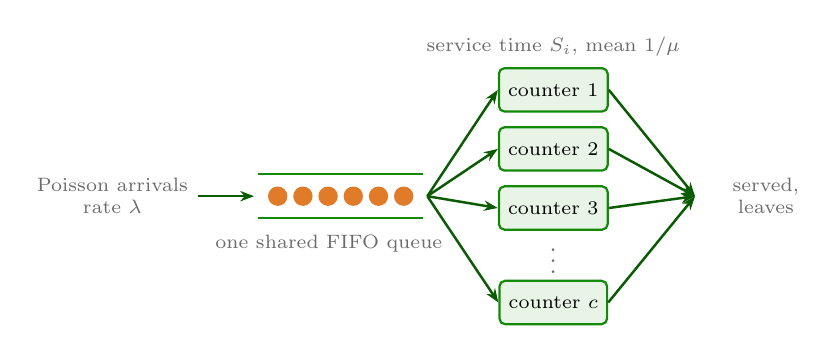
\begin{tikzpicture}[font=\small]
  \node[align=center, color=mute, font=\scriptsize] (src) at (0,0) {Poisson arrivals\\rate $\lambda$};
  \foreach \i in {0,...,5} \node[pax] at (2.1+\i*0.32, 0) {};
  \draw[ovgreen, line width=.8pt] (1.85,-.28) -- (3.95,-.28) (1.85,.28) -- (3.95,.28);
  \node[font=\scriptsize, color=mute] at (2.75,-.6) {one shared FIFO queue};
  \draw[arr] (src.east) -- (1.8,0);
  \foreach \k/\y in {1/1.35, 2/.6, 3/-.15, c/-1.35} {
    \node[lane] (l\k) at (5.6,\y) {counter $\k$};
    \draw[arr] (4.0,0) -- (l\k.west);
    \draw[arr] (l\k.east) -- (7.4,0);
  }
  \node[color=mute] at (5.6,-.72) {$\vdots$};
  \node[align=center, color=mute, font=\scriptsize] at (8.3,0) {served,\\leaves};
  \node[font=\scriptsize, color=mute] at (5.6,1.9) {service time $S_i$, mean $1/\mu$};
\end{tikzpicture}}

% Event loop of the simulator.
\newcommand{\eventdiagram}{%
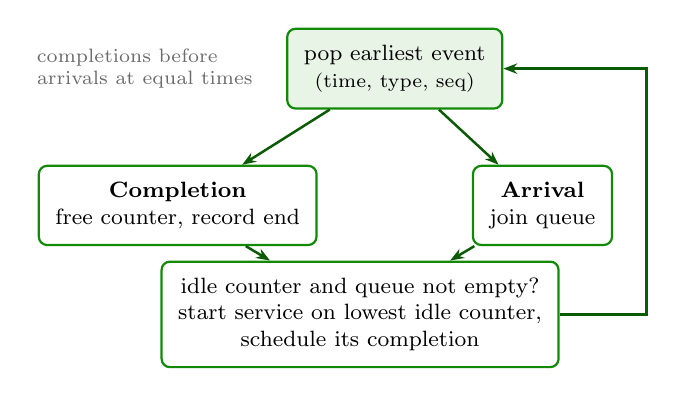
\begin{tikzpicture}[font=\footnotesize, node distance=6mm]
  \node[gbox] (pop) {pop earliest event\\\scriptsize(time, type, seq)};
  \node[box, below left=7mm and -4mm of pop] (cmp) {\textbf{Completion}\\free counter, record end};
  \node[box, below right=7mm and -4mm of pop] (arv) {\textbf{Arrival}\\join queue};
  \node[box, below=7mm of $(cmp)!.5!(arv)$] (start) {idle counter and queue not empty?\\start service on lowest idle counter,\\schedule its completion};
  \draw[arr] (pop) -- (cmp); \draw[arr] (pop) -- (arv);
  \draw[arr] (cmp) -- (start); \draw[arr] (arv) -- (start);
  \draw[arr] (start.east) -- ++(1.1,0) |- (pop.east);
  \node[font=\scriptsize, color=mute, align=left, left=3mm of pop] {completions before\\arrivals at equal times};
\end{tikzpicture}}

% Engine and UI layers.
\newcommand{\archdiagram}{%
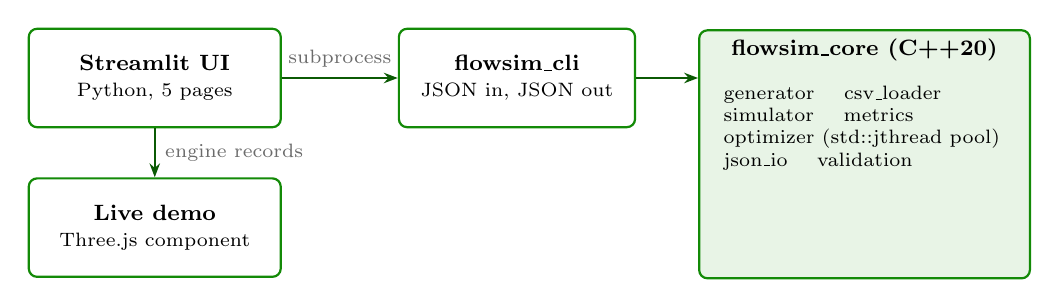
\begin{tikzpicture}[font=\footnotesize]
  \node[box, minimum width=3.2cm, minimum height=1.25cm] (ui) at (0,0) {\textbf{Streamlit UI}\\\scriptsize Python, 5 pages};
  \node[box, minimum width=3.2cm, minimum height=1.25cm] (live) at (0,-1.9) {\textbf{Live demo}\\\scriptsize Three.js component};
  \node[box, minimum width=3.0cm, minimum height=1.25cm] (cli) at (4.6,0) {\textbf{flowsim\_cli}\\\scriptsize JSON in, JSON out};
  \node[gbox, minimum width=4.2cm, minimum height=3.15cm, anchor=north west] (core) at (6.9,.62) {};
  \node[anchor=north, font=\footnotesize\bfseries] at (core.north) {flowsim\_core (C++20)};
  \node[font=\scriptsize, align=left, anchor=north west] at ([shift={(2mm,-6mm)}]core.north west)
    {generator \quad csv\_loader\\simulator \quad metrics\\optimizer (std::jthread pool)\\json\_io \quad validation};
  \draw[arr] (ui.east) -- node[above, font=\scriptsize, color=mute] {subprocess} (cli.west);
  \draw[arr] (cli.east) -- (cli.east -| core.west);
  \draw[arr] (ui) -- node[right, font=\scriptsize, color=mute] {engine records} (live);
\end{tikzpicture}}

% Stacked cost per staffing level.
\newcommand{\costchart}[2]{%
\begin{tikzpicture}
\begin{axis}[fs axis, width=#1, height=#2, ybar stacked, bar width=14pt, ymin=0, ymax=16500,
    xlabel={counters $c$}, ylabel={mean cost per run (INR)}, xtick={3,...,8}, xmin=2.4, xmax=8.6,
    restrict x to domain=3:8, scaled y ticks=false, yticklabel={\pgfmathprintnumber[1000 sep={,}]{\tick}},
    legend columns=3, legend style={at={(0.5,1.02)}, anchor=south}, area legend]
  \addplot[fill=ovgreen, draw=none] table[x=c, y=staffing, col sep=comma] {data/per_counter.csv};
  \addplot[fill=wait, draw=none] table[x=c, y=waiting, col sep=comma] {data/per_counter.csv};
  \addplot[fill=late, draw=none] table[x=c, y=sla, col sep=comma] {data/per_counter.csv};
  \legend{staffing, waiting, SLA penalty}
\end{axis}
\begin{axis}[width=#1, height=#2, ymin=0, ymax=16500, xmin=2.4, xmax=8.6, hide axis]
  \addplot[only marks, mark=*, mark size=1.6pt, ink] table[x=c, y=total, col sep=comma, restrict x to domain=3:8] {data/per_counter.csv};
  \node[font=\scriptsize\bfseries, color=ovdark] at (axis cs:6,8300) {best};
  \node[font=\scriptsize, color=today] at (axis cs:4,11800) {today};
\end{axis}
\end{tikzpicture}}

% People waiting over time in the representative run.
\newcommand{\queuechart}[2]{%
\begin{tikzpicture}
\begin{axis}[fs axis, width=#1, height=#2, xmin=0, xmax=295, ymin=0, xlabel={minutes since 06:00},
    ylabel={people in line}, xtick={0,60,...,300}, legend style={at={(0.02,0.98)}, anchor=north west}]
  \addplot[const plot, today, line width=1pt] table[x=t, y=q, col sep=comma] {data/queue_today.csv};
  \addplot[const plot, ovgreen, line width=1pt] table[x=t, y=q, col sep=comma] {data/queue_plan.csv};
  \legend{{today, 4 lanes},{FlowSim, 6 lanes}}
\end{axis}
\end{tikzpicture}}

% Best counter count against arrival rate.
\newcommand{\sensitivitychart}[2]{%
\begin{tikzpicture}
\begin{axis}[fs axis, width=#1, height=#2, xlabel={arrivals per hour $\lambda$}, ylabel={best counters $c^\ast$},
    ymin=0, ymax=8, xtick={20,28,...,64}, ytick={0,...,8}, axis y line*=left]
  \addplot[const plot mark mid, ovgreen, line width=1.1pt, mark=*, mark size=1.5pt] table[x=rate, y=best, col sep=comma] {data/sensitivity.csv};
  \addplot[dashed, mute, domain=20:64] {x/60*5.5};
  \node[font=\scriptsize, color=mute, rotate=24] at (axis cs:56,4.4) {offered load $\lambda/\mu$};
\end{axis}
\end{tikzpicture}}


\usefonttheme{professionalfonts}
\setbeamertemplate{navigation symbols}{}
\setbeamercolor{structure}{fg=ovgreen}
\setbeamercolor{normal text}{fg=ink}
\setbeamercolor{frametitle}{fg=ovgreen}
\setbeamercolor{title}{fg=ovgreen}
\setbeamercolor{alerted text}{fg=ovdark}
\setbeamerfont{frametitle}{size=\Large, series=\bfseries}
\setbeamertemplate{frametitle}{\vskip6pt\insertframetitle\par\vskip2pt{\color{ovgreen}\rule{\textwidth}{.6pt}}}
\setbeamertemplate{footline}{\hfill{\scriptsize\color{mute}\insertframenumber\hspace{8pt}}\vskip5pt}
\setbeamertemplate{itemize items}{\textcolor{ovgreen}{\tiny$\blacksquare$}}
\setbeamertemplate{section in toc}{\textcolor{ovgreen}{\bfseries\inserttocsectionnumber.}~\inserttocsection}
\setbeamertemplate{note page}{\vskip4pt\insertslideintonotes{0.27}\par\vskip2pt\footnotesize\insertnote}
\setbeamerfont{note page}{size=\footnotesize}

\newcommand{\stat}[2]{\begin{minipage}[t]{.3\linewidth}\centering{\Huge\bfseries\color{ovgreen}#1}\\[2pt]{\small\color{mute}#2}\end{minipage}}
\newcommand{\shot}[2][.92]{\begin{center}\includegraphics[width=#1\linewidth]{figures/#2}\end{center}}

\title{FlowSim}
\subtitle{Simulation-based staffing for service counters}
\author{Sarthak Panda \quad 2022CS51217}
\institute{MSL304 Course Project}
\date{}

\begin{document}

\begin{frame}[plain]
  \vfill
  {\Huge\bfseries\color{ovgreen}FlowSim}\par\vskip4pt
  {\Large Simulation-based staffing for service counters}\par\vskip10pt
  {\color{ovgreen}\rule{.45\textwidth}{.8pt}}\par\vskip10pt
  Sarthak Panda \quad 2022CS51217\par
  {\color{mute}MSL304 Course Project}
  \vfill
  \note{
  \begin{itemize}
    \item Good morning. I am Sarthak Panda, and this is FlowSim, my MSL304 project.
    \item One line: FlowSim decides how many service counters to open by simulating every customer and picking the
      cheapest plan, where cost counts both staff and customers' waiting time.
    \item The running example is an airport security checkpoint during the morning rush.
  \end{itemize}}
\end{frame}

\begin{frame}{Contents}
  \begin{columns}[T]
    \column{.5\textwidth}
    \tableofcontents[sections={1-4}]
    \column{.5\textwidth}
    \tableofcontents[sections={5-8}]
  \end{columns}
  \note{
  \begin{itemize}
    \item The talk has eight short parts: the problem, the model, how the simulation and the search work,
      results on the sample data, the implementation, the platform, a live demo, and conclusions.
    \item The live demo comes near the end, once the audience knows what to look for.
  \end{itemize}}
\end{frame}

\section{Problem}
\begin{frame}{How many lanes should be open?}
  \begin{columns}[c]
    \column{.48\textwidth}
    \begin{itemize}\setlength\itemsep{8pt}
      \item Arrivals are random and bunch up at peaks
      \item \textbf{Too few} lanes: the line explodes, passengers miss flights
      \item \textbf{Too many} lanes: staff sit idle, cost goes up
      \item Managers usually guess, or staff for the worst case
    \end{itemize}
    \vskip10pt
    {\color{ovdark}\bfseries Goal: the lane count with the lowest total cost, with waiting priced in.}
    \column{.5\textwidth}
    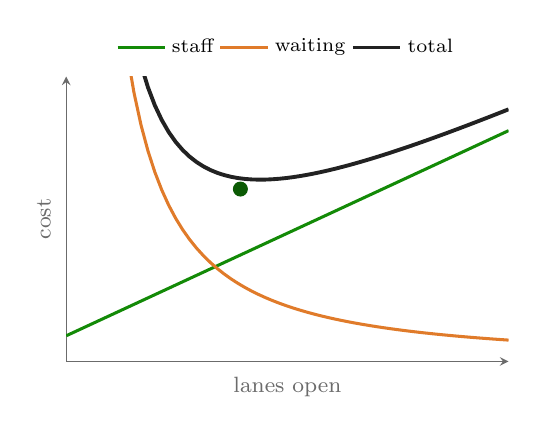
\begin{tikzpicture}
    \begin{axis}[fs axis, width=7.2cm, height=5.2cm, xlabel={lanes open}, ylabel={cost}, xmin=1, xmax=9,
        ymin=0, ymax=10, xtick=\empty, ytick=\empty, legend columns=3, legend style={at={(0.5,1.03)}, anchor=south}]
      \addplot[ovgreen, line width=1.1pt, domain=1:9] {0.9*x};
      \addplot[today, line width=1.1pt, domain=1.6:9, samples=60] {14/(x-0.9)^1.4};
      \addplot[ink, line width=1.4pt, domain=1.6:9, samples=60] {0.9*x + 14/(x-0.9)^1.4};
      \legend{staff, waiting, total}
      \addplot[only marks, mark=*, mark size=2.5pt, ovdark] coordinates {(4.15,6.05)};
    \end{axis}
    \end{tikzpicture}
  \end{columns}
  \note{
  \begin{itemize}
    \item Think of airport security at 6 am. Passengers do not arrive evenly, they come in bursts.
    \item If we open too few lanes, the line grows faster than we can clear it and people miss flights.
    \item If we open every lane, the line disappears, but we pay staff to stand around.
    \item The chart is the whole idea: staff cost rises with each lane, waiting cost falls, and the total has a
      lowest point. FlowSim finds that point using simulation instead of guesswork.
  \end{itemize}}
\end{frame}

\begin{frame}{What FlowSim does}
  \centering
  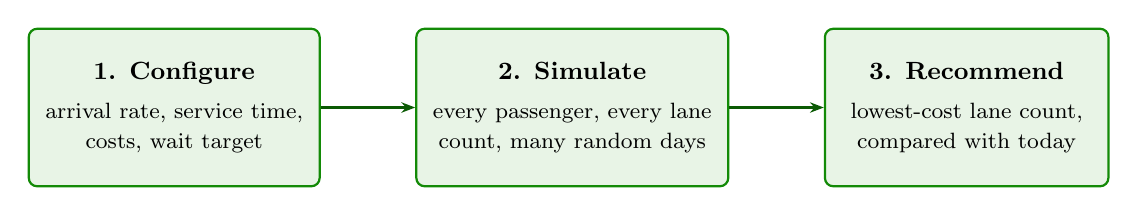
\begin{tikzpicture}[font=\small, node distance=12mm]
    \node[gbox, minimum width=3.6cm, minimum height=2cm] (a) {\textbf{1. Configure}\\[3pt]\footnotesize arrival rate, service time,\\\footnotesize costs, wait target};
    \node[gbox, minimum width=3.6cm, minimum height=2cm, right=of a] (b) {\textbf{2. Simulate}\\[3pt]\footnotesize every passenger, every lane\\\footnotesize count, many random days};
    \node[gbox, minimum width=3.6cm, minimum height=2cm, right=of b] (c) {\textbf{3. Recommend}\\[3pt]\footnotesize lowest-cost lane count,\\\footnotesize compared with today};
    \draw[arr] (a) -- (b); \draw[arr] (b) -- (c);
  \end{tikzpicture}
  \vskip22pt
  \begin{tabular}{@{}ll@{}}
    \color{ovgreen}\bfseries Input & synthetic arrivals or a real passenger CSV \\[3pt]
    \color{ovgreen}\bfseries Output & recommended counters, waits, service level, cost breakdown \\[3pt]
    \color{ovgreen}\bfseries Engine & C++20 discrete-event simulator, Python UI on top
  \end{tabular}
  \note{
  \begin{itemize}
    \item The workflow has three steps.
    \item Configure: describe demand and costs. How many passengers per hour, how long a check takes, what a lane
      costs per hour, what a minute of waiting costs, and the target wait.
    \item Simulate: the engine plays out every passenger for every candidate lane count, over several random days.
    \item Recommend: it picks the cheapest lane count and compares it with what the airport does today.
    \item Input can be generated or uploaded as a CSV of real arrivals.
  \end{itemize}}
\end{frame}

\section{Mathematical model}
\begin{frame}{Queue model}
  \centering\queuediagram
  \vskip4pt
  \begin{columns}[T]
    \column{.47\textwidth}\small
    \begin{itemize}
      \item Arrivals: Poisson, $A_{i+1}-A_i \sim \mathrm{Exp}(\lambda)$
      \item Service: exponential or fixed, mean $1/\mu$
      \item $c$ identical counters, constant all run
    \end{itemize}
    \column{.47\textwidth}\small
    \begin{itemize}
      \item First come, first served; lowest idle counter
      \item No balking, reneging or breaks
      \item Run drains: counters stay until the queue is empty
    \end{itemize}
  \end{columns}
  \note{
  \begin{itemize}
    \item This is the queue we model: one shared line feeding $c$ identical lanes, like most security checkpoints.
    \item Arrivals follow a Poisson process, so the gaps between passengers are exponential with rate lambda.
      Service times are exponential or fixed, with mean one over mu.
    \item In queueing notation this is an M/M/c queue, or G/G/c when we replay real data from a CSV.
    \item The run continues after the last arrival until everyone is served, and we pay staff for that time too.
  \end{itemize}}
\end{frame}

\begin{frame}{Objective}
  For each candidate $c$, a run gives waits $W_i = B_i - A_i$ (start of service minus arrival) and finish time $T$.
  \vskip6pt
  \begin{block}{}
  \[
    c^\ast = \arg\min_{c_{\min}\le c\le c_{\max}} \;\mathbb{E}\Big[
      \underbrace{\frac{c\, r_s\, T}{60}}_{\text{staffing}} +
      \underbrace{\frac{r_w}{60}\sum_i W_i}_{\text{waiting}} +
      \underbrace{p\,\big|\{i : W_i > S\}\big|}_{\text{SLA penalty}}\Big]
  \]
  \end{block}
  \vskip4pt
  \small
  \begin{tabular}{@{}lll@{\qquad}lll@{}}
    \toprule
    $r_s$ & cost per counter-hour & 250 & $S$ & wait target (min) & 10 \\
    $r_w$ & cost per waiting passenger-hour & 35 & $p$ & penalty per late passenger & 20 \\
    $T$ & last service completion (min) & & $\mathbb{E}$ & mean over $R$ replications & $R=10$ \\
    \bottomrule
  \end{tabular}
  \note{
  \begin{itemize}
    \item This is the mathematical heart of the project.
    \item For each lane count $c$ we simulate, measure every passenger's wait $W_i$, and add up three costs.
    \item Staffing: $c$ lanes times the hourly rate times the hours they are open, including the drain at the end.
    \item Waiting: total passenger-hours spent in line, times a value of time.
    \item SLA penalty: a fixed charge for every passenger who waited longer than the 10 minute target. Note the
      strict greater-than.
    \item Because the system is random, we take the expectation, estimated as the mean over $R$ simulated days,
      and pick the $c$ with the smallest mean. Ties go to fewer lanes.
    \item The numbers in the table are the illustrative values used in the sample scenario.
  \end{itemize}}
\end{frame}

\section{Simulation and search}
\begin{frame}{Discrete-event simulation}
  \begin{columns}[c]
    \column{.55\textwidth}
    \centering\eventdiagram
    \column{.42\textwidth}\small
    \begin{itemize}\setlength\itemsep{6pt}
      \item Jumps from event to event, no time steps
      \item Min-heap of events, min-heap of idle counters
      \item Fixed tie order, so runs are fully deterministic
      \item Safety cap on events stops runaway runs
      \item Cost: $O(n \log n)$ for $n$ passengers
    \end{itemize}
  \end{columns}
  \note{
  \begin{itemize}
    \item The engine is a discrete-event simulator. Instead of ticking a clock every second, it jumps straight to
      the next thing that happens.
    \item Only two event types exist: an arrival and a service completion.
    \item On a completion we free the counter, and if someone is waiting, they start immediately.
    \item On an arrival, the passenger takes the lowest-numbered idle counter or joins the back of the line.
    \item If a completion and an arrival happen at the same instant, the completion is processed first, so the
      arriving passenger can walk straight in with zero wait.
    \item Every tie is broken by a fixed rule, so the same input always gives exactly the same output.
  \end{itemize}}
\end{frame}

\begin{frame}{Searching staffing levels}
  \begin{columns}[T]
    \column{.5\textwidth}
    \textbf{\color{ovgreen}Exhaustive search}
    \begin{itemize}\small
      \item Try every $c$ from $c_{\min}$ to $c_{\max}$
      \item $R$ replications each, seed $s+r$
    \end{itemize}
    \vskip8pt
    \textbf{\color{ovgreen}Common random numbers}
    \begin{itemize}\small
      \item Replication $r$ uses the same passengers for every $c$
      \item Differences come from staffing, not from luck
    \end{itemize}
    \column{.5\textwidth}
    \textbf{\color{ovgreen}Parallel and reproducible}
    \begin{itemize}\small
      \item $(r, c)$ tasks on a \texttt{std::jthread} pool
      \item Each task writes its own slot, no locks
      \item Parallel output identical to sequential
    \end{itemize}
    \vskip8pt
    \textbf{\color{ovgreen}Decision rule}
    \begin{itemize}\small
      \item Lowest mean objective wins
      \item Within $10^{-9}$ relative: fewer counters
    \end{itemize}
  \end{columns}
  \note{
  \begin{itemize}
    \item The search is simple and exact over the range: we try every lane count.
    \item The key statistical trick is common random numbers. Day number one uses the same passengers for 4 lanes,
      5 lanes and 6 lanes. So when 6 beats 4, it is because of staffing, not because 6 happened to get a quieter day.
    \item All replication and lane-count combinations run in parallel on a bounded thread pool. Each task writes
      to its own slot, and the results are combined in a fixed order, so parallel and sequential runs agree to
      the last digit.
  \end{itemize}}
\end{frame}

\section{Results on the sample}
\begin{frame}{Sample scenario: airport morning rush}
  \centering
  \begin{tabular}{@{}lr@{\qquad\qquad}lr@{}}
    \toprule
    Arrival window & 240 min & Counter cost & 250 / hour \\
    Arrival rate $\lambda$ & 48 / hour & Waiting cost & 35 / passenger-hour \\
    Mean service $1/\mu$ & 5.5 min, exponential & Wait target $S$ & 10 min \\
    Today & 4 counters & Late penalty $p$ & 20 / passenger \\
    Candidates & 1 to 8 counters & Replications, seed & 10, 42 \\
    \bottomrule
  \end{tabular}
  \vskip16pt
  Offered load $\lambda/\mu = 48 \times 5.5 / 60 = \mathbf{4.4}$ busy counters on average.\\[3pt]
  {\color{today}\bfseries With 4 counters the line can only grow.}
  \note{
  \begin{itemize}
    \item Here is the sample scenario. The numbers are illustrative, not measured airport data.
    \item 48 passengers an hour for 4 hours, each taking 5.5 minutes on average.
    \item Quick sanity check: 48 times 5.5 divided by 60 is 4.4. On average 4.4 counters must be busy just to
      keep up. The airport opens 4, so the line is mathematically guaranteed to grow through the morning.
    \item Question for the audience: how many lanes would you open? Most people say 5.
  \end{itemize}}
\end{frame}

\begin{frame}{Total cost by staffing level}
  \begin{columns}[c]
    \column{.6\textwidth}
    \costchart{8.6cm}{6.2cm}
    \column{.38\textwidth}
    \stat{6}{recommended\\counters}\hfill\stat{34\%}{cheaper\\than today}
    \vskip14pt\small
    \begin{itemize}
      \item 5 lanes: saves 961 staff, adds 1,017 waiting and penalty
      \item 7 lanes: adds 1,018 staff to save 149
      \item $c=1,2$ off the chart (26k to 58k)
    \end{itemize}
  \end{columns}
  \note{
  \begin{itemize}
    \item This is the U-shaped curve from the first slide, now with real engine numbers.
    \item Dark green is staffing, light green is waiting, red is the late penalty. Black dots are the totals.
    \item At 4 lanes, today, waiting and penalties dominate. At 6 they almost vanish.
    \item Why not 5? Five saves about 961 in staff but adds about 1,017 in waiting and penalties, so it is
      slightly worse. Why not 7? It costs 1,018 more in staff to save only 149.
    \item So 6 is the minimum, and it is 34 percent cheaper on average than today's 4.
  \end{itemize}}
\end{frame}

\begin{frame}{Results table (mean of 10 replications)}
  \centering\small
  \pgfplotstabletypeset[col sep=comma,
    columns={c,total,sd,wait,p95,service_level,util,maxq},
    columns/c/.style={column name={$c$}, int detect},
    columns/total/.style={column name={cost}, fixed, precision=0, 1000 sep={,}},
    columns/sd/.style={column name={sd}, fixed, precision=0, 1000 sep={,}},
    columns/wait/.style={column name={wait (min)}, fixed, precision=2, zerofill},
    columns/p95/.style={column name={p95 wait}, fixed, precision=1, zerofill},
    columns/service_level/.style={column name={on time \%}, fixed, precision=1, zerofill},
    columns/util/.style={column name={utilization \%}, fixed, precision=1, zerofill},
    columns/maxq/.style={column name={max line}, fixed, precision=1, zerofill},
    every head row/.style={before row=\toprule, after row=\midrule},
    every last row/.style={after row=\bottomrule},
    every row no 3/.style={before row={\rowcolor{today!14}}},
    every row no 5/.style={before row={\rowcolor{ovlight}}},
  ]{data/per_counter.csv}
  \vskip8pt
  {\scriptsize\color{mute}orange: today (4) \quad green: recommended (6) \quad costs in INR per 4 hour run}
  \note{
  \begin{itemize}
    \item The same results as a table, averaged over 10 simulated mornings.
    \item Today, with 4 lanes: average wait about 20 minutes, the 95th percentile around 36 minutes, and only
      a third of passengers on time.
    \item With 6 lanes: average wait about 1.2 minutes and almost 99 percent on time. Utilization drops from 95
      to about 72 percent, which is a healthy level.
    \item The sd column is the spread across days. It shows why we average over replications instead of trusting
      one run.
  \end{itemize}}
\end{frame}

\begin{frame}{Same passengers, two plans}
  \begin{columns}[c]
    \column{.6\textwidth}
    \queuechart{8.6cm}{6cm}
    \column{.38\textwidth}\small
    \pgfplotstableread[col sep=comma]{data/rep_run.csv}\rep
    \begin{tabular}{@{}lrr@{}}
      \toprule
      replication 0 & \color{today}today & \color{ovgreen}FlowSim \\
      \midrule
      counters & 4 & 6 \\
      mean wait (min) & 18.7 & 0.9 \\
      max line & 33 & 9 \\
      on time \% & 31.1 & 100 \\
      total cost & 10,010 & 6,543 \\
      \bottomrule
    \end{tabular}
  \end{columns}
  \note{
  \begin{itemize}
    \item One representative morning, the same 199 passengers, played through both plans.
    \item The orange line is today's queue: it climbs for the whole four hours and peaks above 30 people.
    \item The green line, with 6 lanes, never goes above 9 and is usually near zero.
    \item The table on the right is this single morning. Today's plan cost 10,010; the recommended plan cost
      6,543, even though it pays for two extra lanes.
    \item This is exactly what the live demo animates.
  \end{itemize}}
\end{frame}

\begin{frame}{Does the engine agree with queueing theory?}
  \begin{columns}[c]
    \column{.5\textwidth}
    \centering\small
    M/M/$c$, one week ($10{,}080$ min), 20 replications
    \vskip6pt
    \pgfplotstabletypeset[col sep=comma, columns={c,rho,sim,theory,err_pct},
      columns/c/.style={column name={$c$}, int detect},
      columns/rho/.style={column name={$\rho$}, fixed, precision=2, zerofill},
      columns/sim/.style={column name={simulated $W_q$}, fixed, precision=3, zerofill},
      columns/theory/.style={column name={Erlang C $W_q$}, fixed, precision=3, zerofill},
      columns/err_pct/.style={column name={diff \%}, fixed, precision=1, zerofill},
      every head row/.style={before row=\toprule, after row=\midrule}, every last row/.style={after row=\bottomrule}]
      {data/erlang.csv}
    \vskip6pt
    {\scriptsize\color{mute}within 2\% of the closed form}
    \column{.48\textwidth}
    \centering\small Best $c^\ast$ as demand grows
    \sensitivitychart{7cm}{5.2cm}
  \end{columns}
  \note{
  \begin{itemize}
    \item Two checks that the model behaves sensibly.
    \item Left: for a long run, the M/M/c queue has an exact formula for the mean wait, the Erlang C formula. The
      simulated waits match it within 2 percent for every lane count. This validates the engine.
    \item Right: as arrivals per hour go up, the recommended lane count rises in steps and always stays above the
      dashed offered-load line. That is the rule of thumb from queueing theory: you need spare capacity.
  \end{itemize}}
\end{frame}

\section{Implementation}
\begin{frame}{Architecture}
  \centering\archdiagram
  \vskip14pt
  \begin{columns}[T]
    \column{.31\textwidth}\small
    \textbf{\color{ovgreen}C++20 engine}\\ all simulation, metrics and the optimizer; Python never simulates
    \column{.31\textwidth}\small
    \textbf{\color{ovgreen}Strict contract}\\ versioned JSON schema, field-level errors, exit codes 0 to 4
    \column{.31\textwidth}\small
    \textbf{\color{ovgreen}Python UI}\\ Streamlit, Plotly charts, Three.js replay of real engine events
  \end{columns}
  \note{
  \begin{itemize}
    \item The C++20 engine is the single source of truth. It generates passengers, simulates, computes metrics
      and runs the optimizer.
    \item The Streamlit UI writes a JSON scenario, calls the command line tool as a subprocess without a shell,
      and reads JSON back. Python never computes a metric itself.
    \item The live demo is a custom Three.js component. It replays the exact arrival, start and end times and the
      counter the engine reported for each passenger.
    \item Bad input is rejected with an error naming the exact field.
  \end{itemize}}
\end{frame}

\begin{frame}{Engineering and testing}
  \begin{columns}[T]
    \column{.48\textwidth}
    \begin{itemize}\small\setlength\itemsep{5pt}
      \item 33 C++ unit tests: FIFO, ties, hand-computed metrics, CRN, parallel = sequential
      \item 35 Python tests drive every UI page against the real engine
      \item AddressSanitizer, UBSan and ThreadSanitizer builds
      \item GitHub Actions CI on every pull request
    \end{itemize}
    \column{.5\textwidth}
    \centering\small
    Benchmark: 32 runs on 8 vCPU
    \vskip6pt
    \begin{tabular}{@{}rrrr@{}}
      \toprule
      passengers & sequential & 8 threads & speedup \\
      \midrule
      1,007 & 3.5 ms & 0.9 ms & 3.9$\times$ \\
      9,998 & 32.4 ms & 4.7 ms & 6.9$\times$ \\
      99,838 & 363.6 ms & 43.7 ms & 8.3$\times$ \\
      \bottomrule
    \end{tabular}
  \end{columns}
  \note{
  \begin{itemize}
    \item The engine is tested like production code.
    \item Unit tests cover the tricky cases: simultaneous events, FIFO order, metrics checked by hand, and the
      guarantee that parallel and sequential runs give identical numbers.
    \item The Python tests open every page of the app and call the real engine.
    \item Sanitizer builds check for memory errors and data races, and all of this runs automatically in CI.
    \item Performance: about 100 thousand passengers across 32 simulations in under 50 milliseconds with 8 threads.
  \end{itemize}}
\end{frame}

\section{The platform}
\begin{frame}{Live demo screen}
  \shot[.86]{live_demo.png}
  \note{
  \begin{itemize}
    \item This is the landing screen after pressing Load sample and simulate.
    \item Left hall: today's 4 lanes. Right hall: FlowSim's 6 lanes. Same passengers arrive at both.
    \item The ring under each passenger shows their wait: green on time, amber close to the target, red late.
    \item The boards above each hall and the two charts below update live: people in line and cost so far.
  \end{itemize}}
\end{frame}

\begin{frame}{Build a scenario, simulate a plan}
  \begin{columns}[T]
    \column{.49\textwidth}\centering
    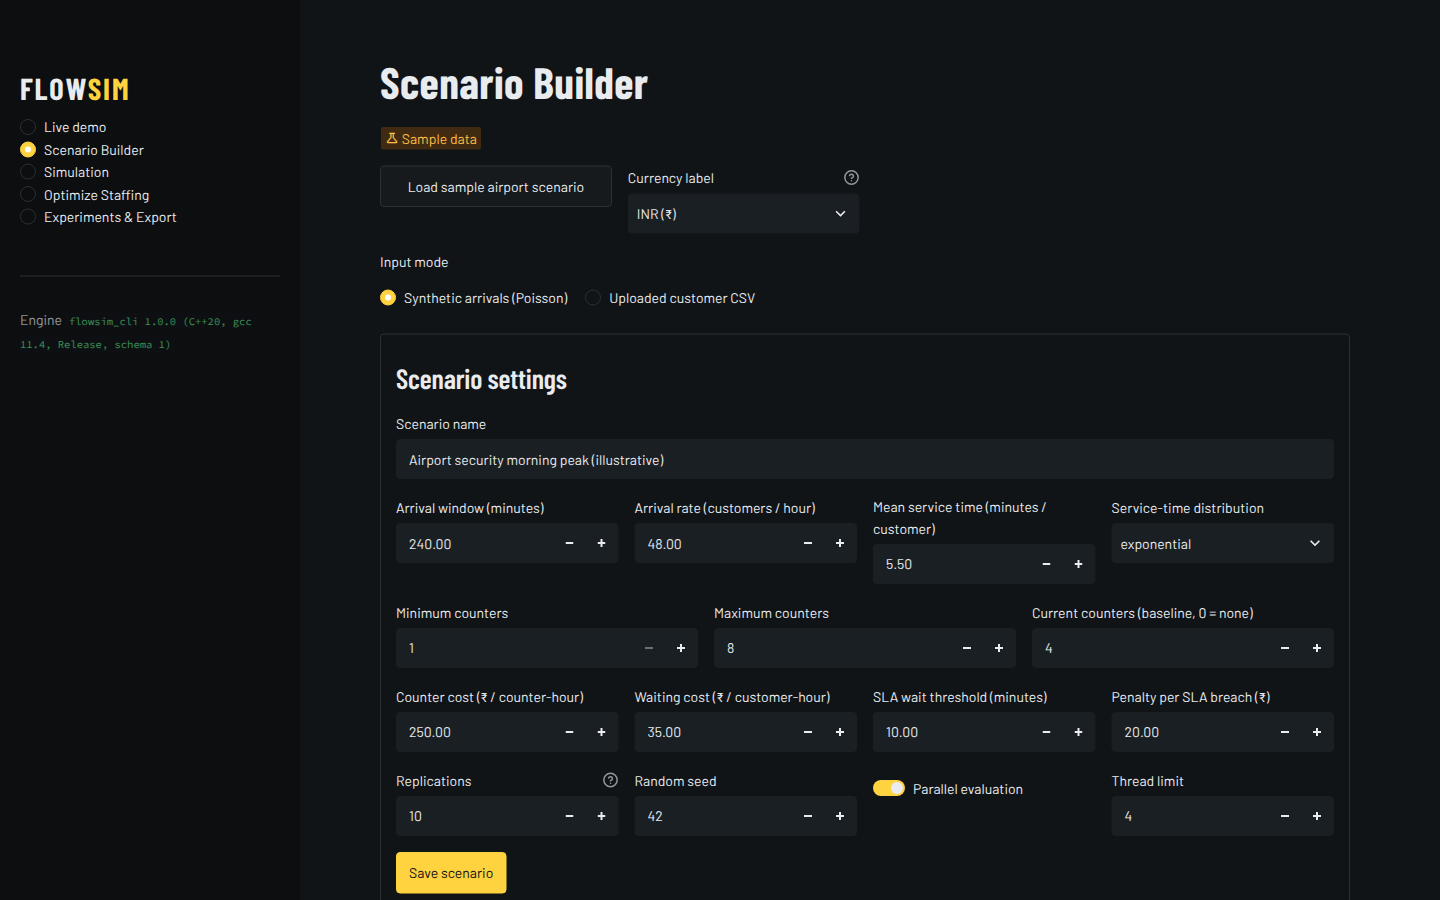
\includegraphics[width=\linewidth]{figures/scenario_builder.png}\\[4pt]
    \textbf{Scenario Builder}\\\small synthetic Poisson data or a passenger CSV, checked field by field
    \column{.49\textwidth}\centering
    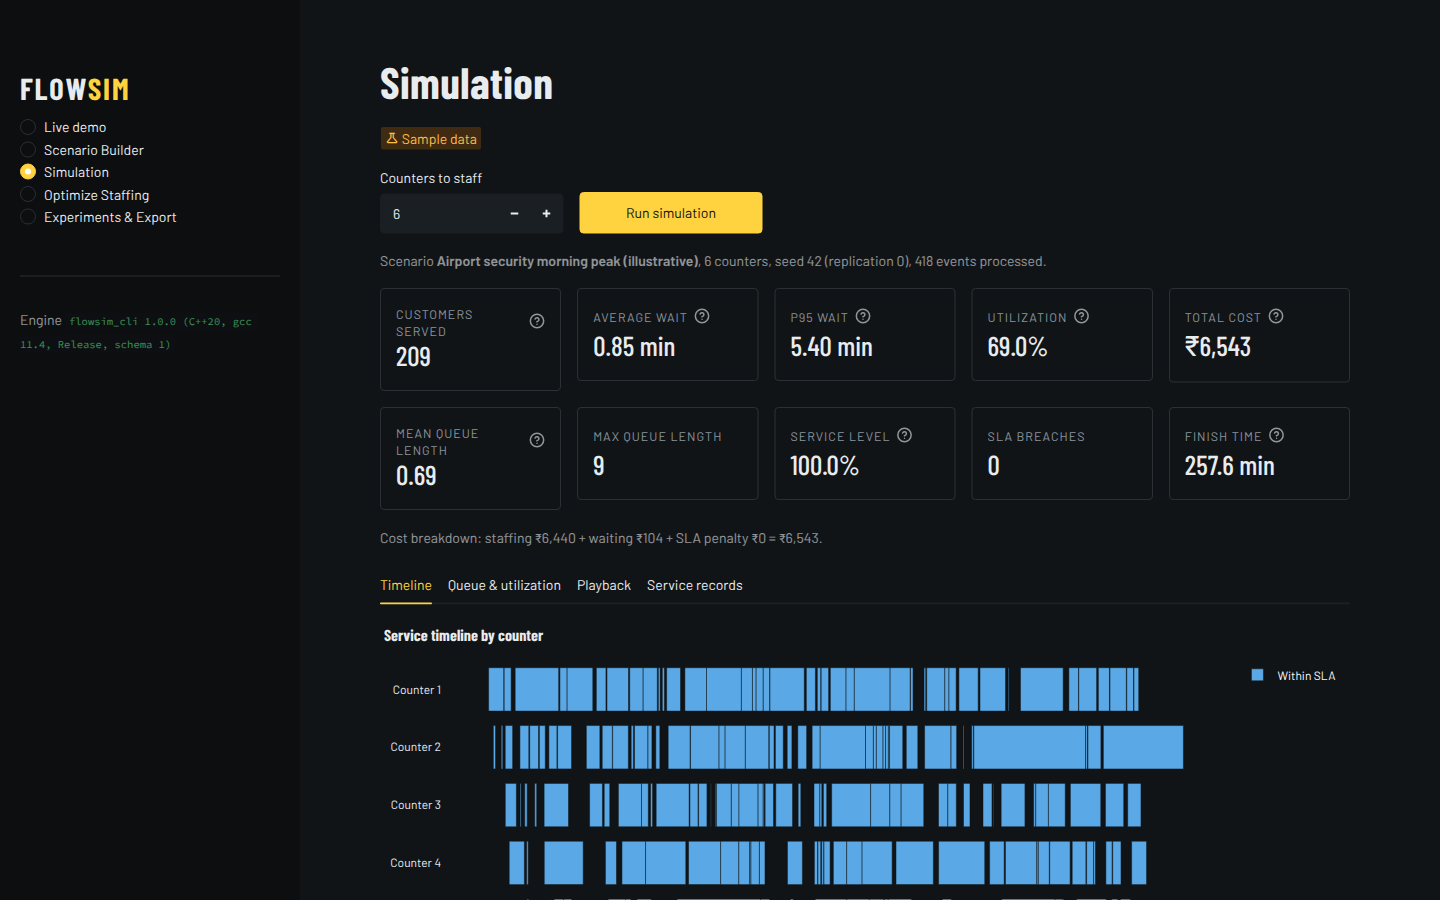
\includegraphics[width=\linewidth]{figures/simulation.png}\\[4pt]
    \textbf{Simulation}\\\small one plan: KPIs, per-passenger timeline, queue and utilization
  \end{columns}
  \note{
  \begin{itemize}
    \item Beyond the demo, the app has the full workflow.
    \item Scenario Builder: generate synthetic arrivals or upload a CSV of real passengers. Inputs are validated
      before anything runs, and the page shows the offered load so you can see at once if a plan cannot keep up.
    \item Simulation: run one plan and inspect it, down to a timeline bar for every passenger and the queue and
      utilization over time.
  \end{itemize}}
\end{frame}

\begin{frame}{Optimize and export}
  \begin{columns}[T]
    \column{.49\textwidth}\centering
    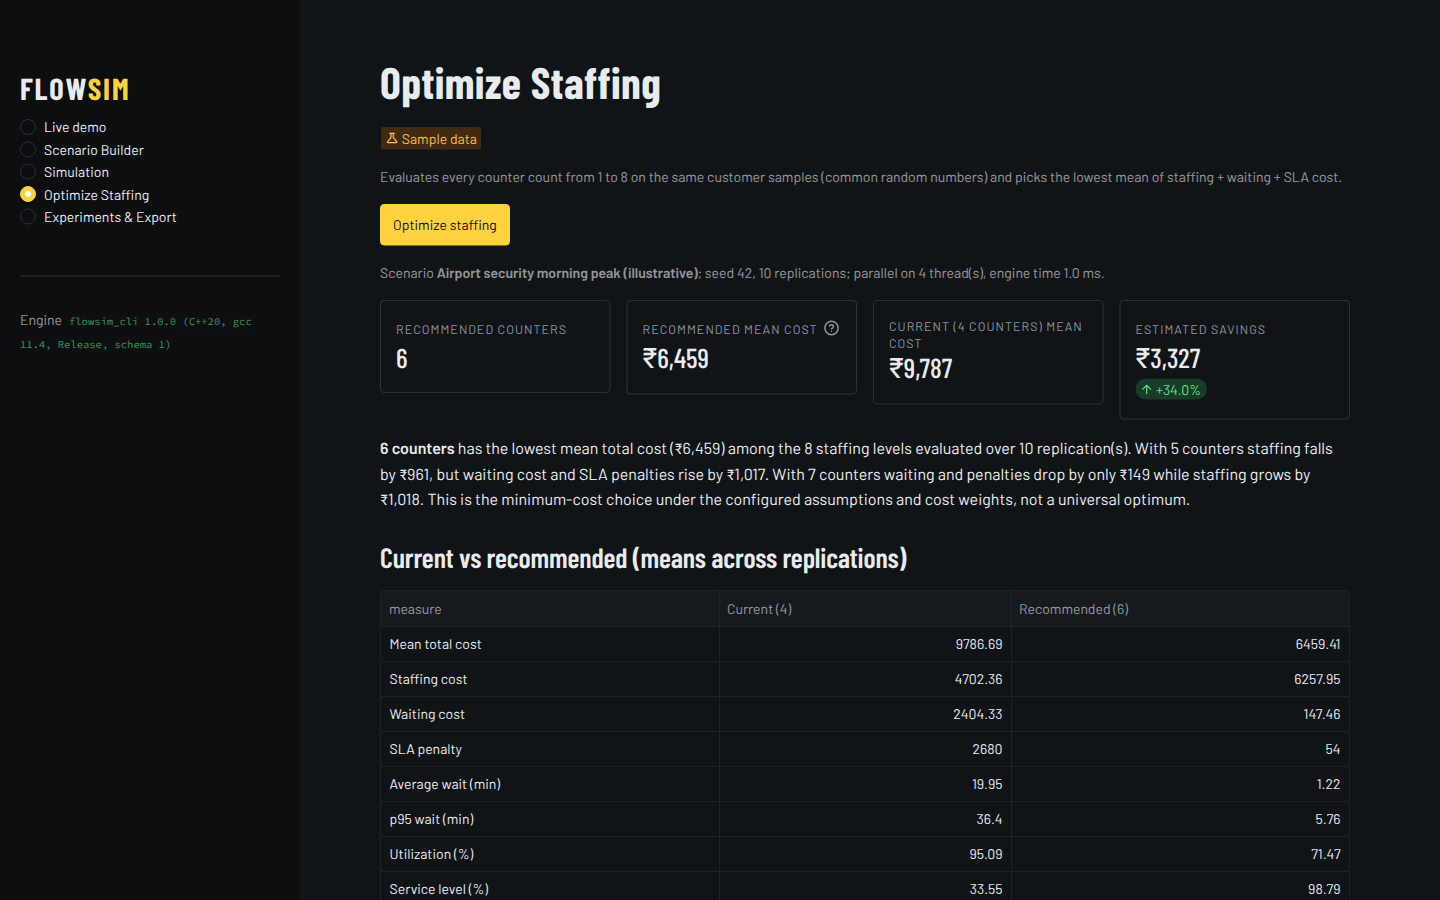
\includegraphics[width=\linewidth]{figures/optimize_staffing.png}\\[4pt]
    \textbf{Optimize Staffing}\\\small every lane count, U-shaped cost chart, plain-language reason
    \column{.49\textwidth}\centering
    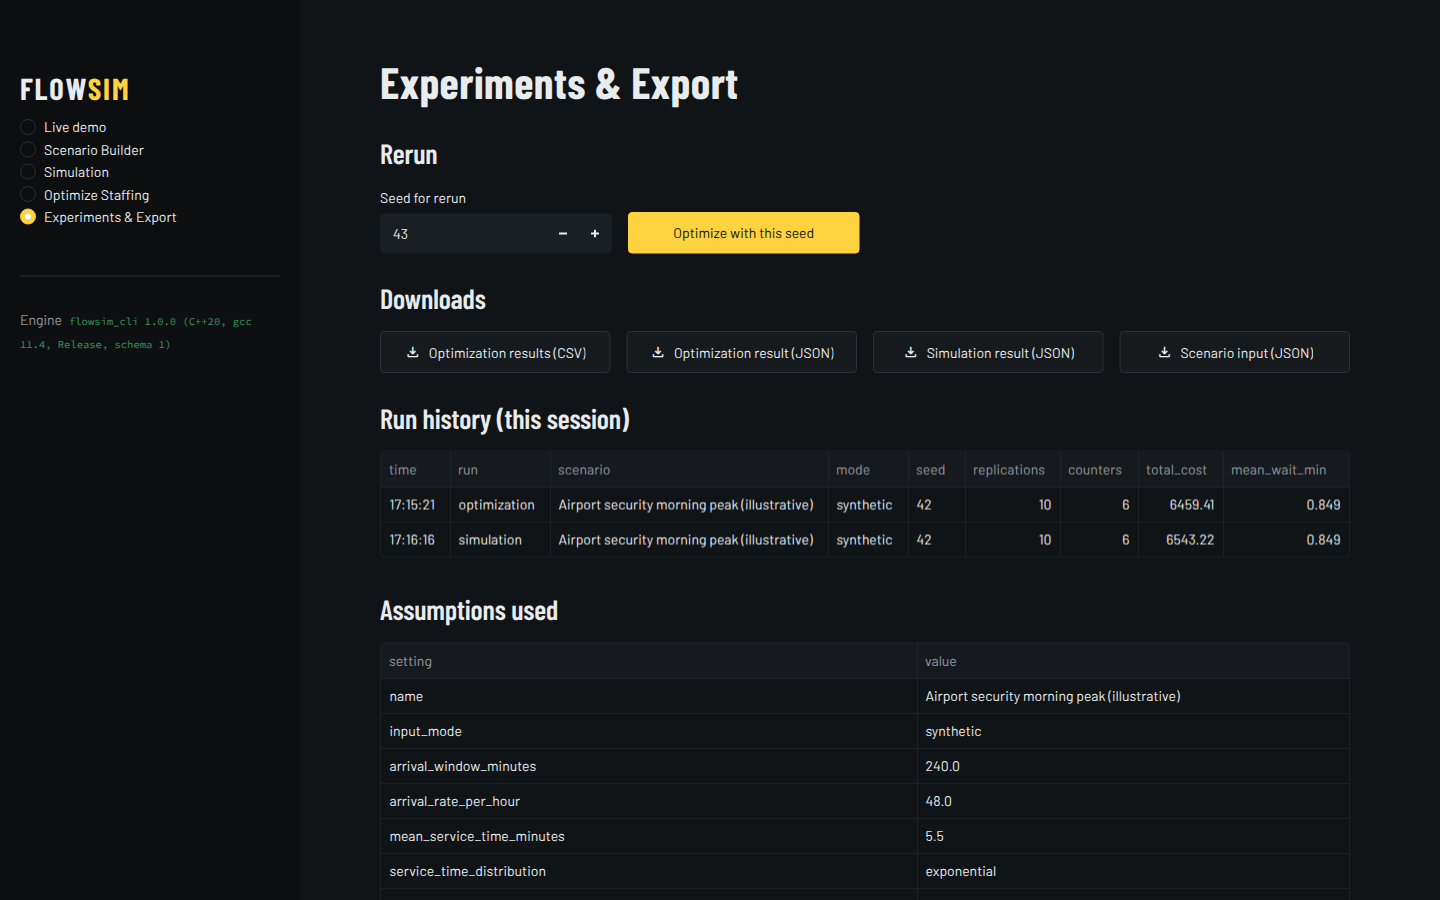
\includegraphics[width=\linewidth]{figures/experiments_export.png}\\[4pt]
    \textbf{Experiments \& Export}\\\small new seeds, run history, CSV and JSON downloads
  \end{columns}
  \note{
  \begin{itemize}
    \item Optimize Staffing sweeps all lane counts, draws the cost curve, and gives a one sentence explanation of
      why the recommendation wins against one lane fewer and one lane more.
    \item Experiments and Export re-runs with a new seed, keeps a history of runs, and downloads the results as CSV
      or JSON for a report.
  \end{itemize}}
\end{frame}

\begin{frame}{What the platform offers}
  \begin{columns}[c]
    \column{.47\textwidth}
    \begin{itemize}\setlength\itemsep{7pt}
      \item \textbf{Synthetic data}: Poisson arrivals, exponential or fixed service, seeded
      \item \textbf{Real data}: upload a passenger CSV
      \item \textbf{Live simulation}: 3D replay, play, pause, scrub, up to 8$\times$
      \item \textbf{Optimization}: cost curve and recommendation
      \item \textbf{Experiments}: seeds, history, export
      \item \textbf{Web replay}: static site on GitHub Pages
    \end{itemize}
    \column{.51\textwidth}
    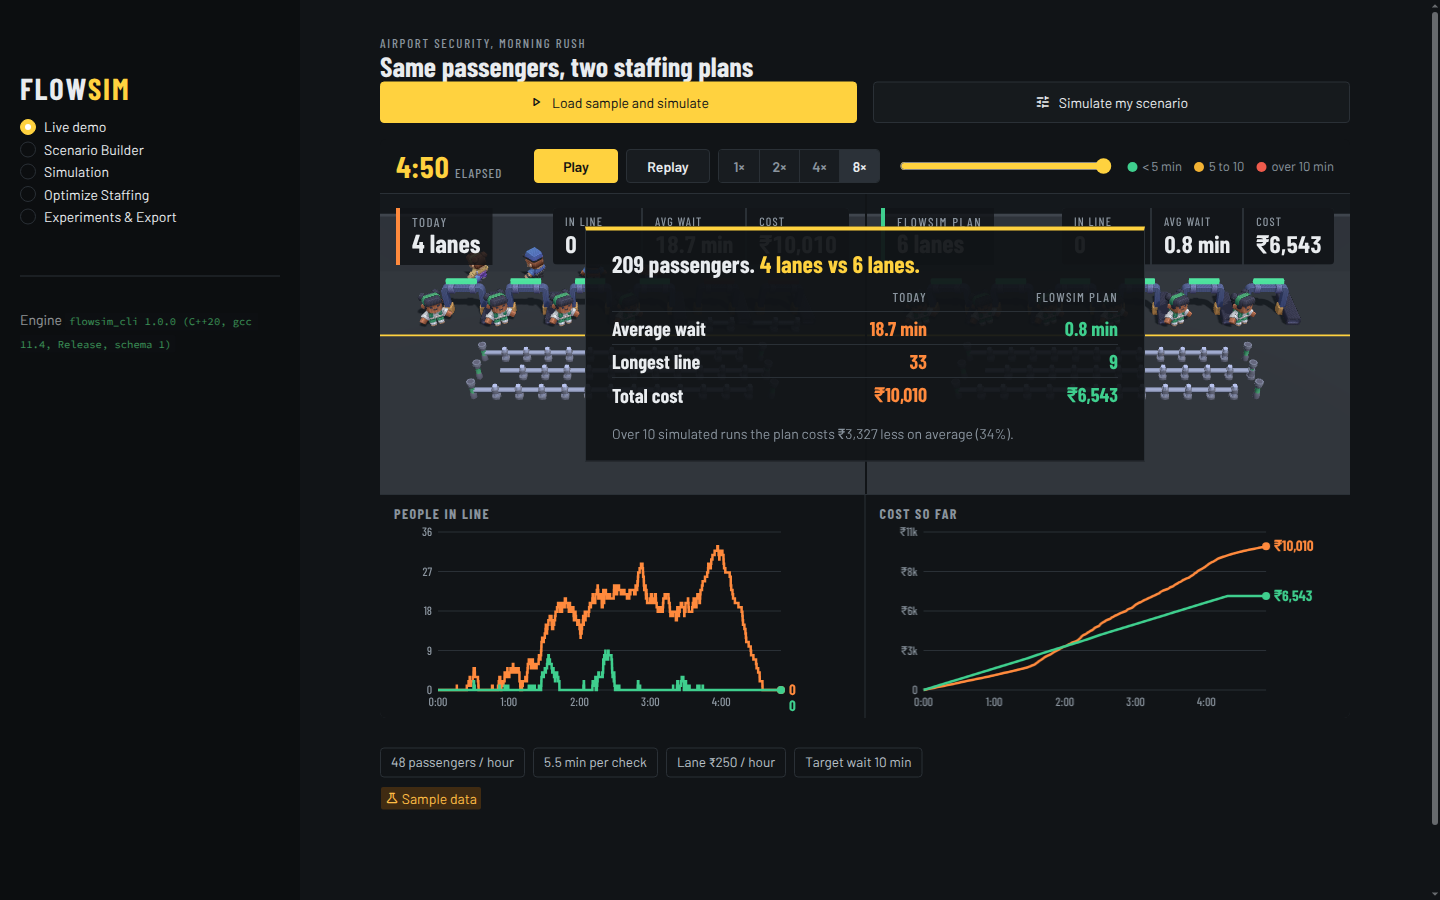
\includegraphics[width=\linewidth]{figures/live_demo_result.png}
  \end{columns}
  \note{
  \begin{itemize}
    \item To summarise the features: two ways to get data in, synthetic or a real CSV.
    \item A live 3D replay you can pause, scrub and speed up. The picture is the result card at the end of a replay.
    \item The optimizer with its explanation, and an experiments page with history and export.
    \item There is also a static web version of the replay that can be hosted on GitHub Pages.
  \end{itemize}}
\end{frame}

\section{Live demo}
\begin{frame}[plain]{}
  \centering\vfill
  \href{http://localhost:8501}{
\begin{tikzpicture}
    \fill[ovgreen] (0,0) circle (1.5cm);
    \fill[white] (-.45,-.75) -- (-.45,.75) -- (.85,0) -- cycle;
  \end{tikzpicture}}
  \vskip16pt
  {\Huge\bfseries\color{ovgreen}Live demo}\par\vskip6pt
  {\color{mute}\href{http://localhost:8501}{localhost:8501}}
  \vfill
  \note{
  \begin{itemize}
    \item Switch to the browser now. Before the talk run ./scripts/run\_demo.sh and keep localhost:8501 open.
    \item Press Load sample and simulate. Point at the left line growing while the right hall keeps up.
    \item Point at Cost so far: the plan starts more expensive because it pays for two extra lanes, and around
      the two hour mark the orange line overtakes it.
    \item Press 8x to reach the end and read the result card: about 18.7 versus 0.8 minutes average wait.
    \item If time allows, change the arrival rate in Scenario Builder and press Simulate my scenario.
  \end{itemize}}
\end{frame}

\section{Conclusion}
\begin{frame}{Conclusion}
  \begin{columns}[T]
    \column{.5\textwidth}
    \textbf{\color{ovgreen}Takeaways}
    \begin{itemize}\small\setlength\itemsep{5pt}
      \item Priced waiting turns staffing into a clear minimum
      \item Sample: 6 lanes instead of 4, \textbf{34\%} cheaper, wait 20 to 1.2 min
      \item Engine matches Erlang C within 2\%
      \item Same passengers on both sides makes the gain easy to see
    \end{itemize}
    \column{.48\textwidth}
    \textbf{\color{ovgreen}Limits and next steps}
    \begin{itemize}\small\setlength\itemsep{5pt}
      \item Constant staffing; next: per time block plans
      \item One shared queue; next: per-lane queues, priority lanes
      \item Illustrative costs; next: calibrate on real data
      \item Exhaustive search; next: local search for large plans
    \end{itemize}
  \end{columns}
  \vskip22pt
  \centering{\Large\bfseries\color{ovgreen}Thank you}\par\vskip2pt
  {\small\color{mute}github.com/sarthak-panda/MSL304-Project}
  \note{
  \begin{itemize}
    \item To conclude: once waiting has a price, the staffing decision has a clear minimum, and simulation finds it.
    \item On the sample, 6 lanes instead of 4 cut cost by about a third and average wait from 20 minutes to about 1.
    \item The engine agrees with queueing theory, and the side-by-side replay makes the result easy to explain.
    \item Limits: staffing is constant for the whole window, there is one shared line, and the costs are
      illustrative. The natural next step is staffing per time block, which the proposal planned, using local
      search when the number of plans grows.
    \item Thank you. I am happy to take questions.
  \end{itemize}}
\end{frame}

\end{document}
